\documentclass{uafthesis}

\usepackage{fixltx2e} % At the least, allows \(\) in captions.
\usepackage{ppl} % Bitches love the Paladino font.
\usepackage{amsmath, amssymb, amsfonts} % Thanks, AMS!
\usepackage{graphicx, float, subfig} % Graphics stuff
%\usepackage{epstopdf} % Should let me include eps images. Requires write18?
\usepackage{verbatim} % Mostly for the comment environment.
%\usepackage{chapterbib} % This is an option for those bundling papers.
\usepackage{minted} % Syntax hilighting!
\usepackage{ulem} % This is mostly for sout.
\usepackage[square]{natbib}
\usepackage{tocbibind} % This fixes the "bibliography in ToC" problem that those
                       % asshole physicists said should be fixed by directly
                       % hacking the .toc file.

%Custom macros go here.

\newcommand{\Ei}{\textrm{Ei}} % Exponential integral
\newcommand{\e}[0]{\hat{e}} % Unit vector
\newcommand{\norm}[1]{\left|\left|{#1}\right|\right|} % |n|


\begin{document}

\title{The Measurement of Anisotropic Thermal Conductivity in Snow With Needle Probes}
\author{Joshua Holbrook}

\degreeyear{2011}
\degreemonth{May}
\degree{Master of Science}
\department{Dept. of Mechanical Engineering}
\numberofmembers{3} % Make sure this is right! The grad school hates empty
                    % signature lines.
\prevdegrees{B.S.}
\college{College of Engineering and Mines}

\makesig
\maketitle

% Wondering when to use `input' and when to use `include?'
% read http://en.wikibooks.org/wiki/LaTeX/Basics#Big_Projects .
\begin{abstract}
  \input abstract.tex
\end{abstract}


%Table of Contents and such
\tableofcontents
\listoffigures
\listoftables
%\listofothermaterials
\listofappendices

\begin{acknowledgements}
  \input acknowledgements.tex
\end{acknowledgements}

\begin{quotepage}
  \input quotepage.tex
\end{quotepage}

\chapter{Introduction}
\label{sec:introduction}
\bigskip

\section{Why Snow's Conductivity Matters}

The thermal properties of snow are of interest to scientists studying Arctic and
sub-Arctic climates because, during the long, cold winters in this region,
snow's thermal behavior plays a critical role in determining the net energy
balance between Earth's surface and the atmosphere. After all, any heat transfer
occurring between the Earth and the atmosphere over snow-covered ground must go
through the snow first (Figure \ref{fig:climate}). In fact, the snow
itself may store and release energy over time.

\begin{figure}[h]
\centering
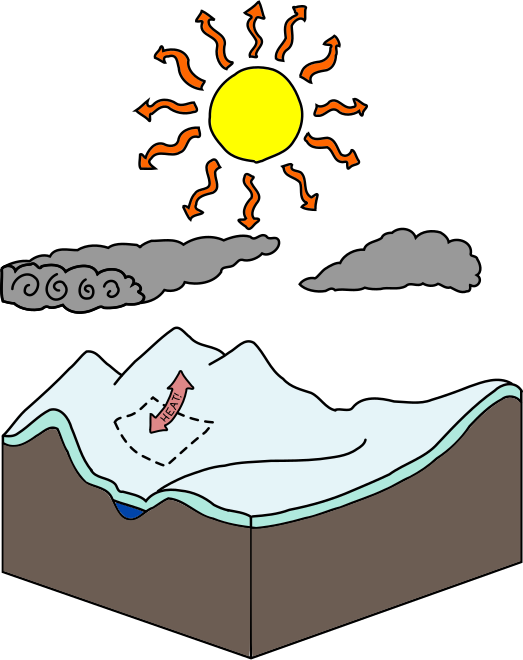
\includegraphics[width=0.4\textwidth]{fig/climate.png}
\caption{Arctic and Sub-Arctic climate is affected largely by heat transfer
between the atmosphere and the ground. Snowpack adds thermal resistance
transfer, affecting this heat transfer.}
\label{fig:climate}
\end{figure}

This energy transfer is critical in accurate climate models for these cold
regions, therefore the effective thermal conductivity of snow is a very
important factor for these models, and has been studied thoroughly. \cite{sturm1,sturm2,sturm3}

\section{Thermal Conductivity Measurements of Snow}

A typical technique for measuring thermal conductivity, especially in the
context of engineering materials such as building insulation, is the guarded
hot plate method. For this technique, a constant temperature gradient is induced across
the material, and heat flux over the material is measured.  By Fourier's Law,
\(k = \frac{\dot{q}l}{A\Delta T}\), where \(\dot{q}\) is the heat flux, \(A\) is
the cross-sectional area of the sample, \(l\) is the sample thickness, and 
\(\Delta T\) is the temperature difference across the sample. This technique
works well in many cases.

Another technique used for porous materials, such as soils and snow, is the
needle probe method. A needle probe consists of a long, thin needle with heating
wire running along its interior, and a temperature sensor in the center. This
configuration approximates an infinite line of constant-flux heat source
(Figure \ref{fig:needle_xsect}). \cite{basictheory}

\begin{figure}[h]
\centering
\includegraphics[width=0.4\textwidth]{fig/needle_xsect.png}
\caption{An illustration of a needle probe in cross-section. Note that the heat
trace in many needle probes, including the one used in experiments for this
research, actually wraps around an inner core instead of running axially through
the needle.}
\label{fig:needle_xsect}
\end{figure}

This needle is inserted into the material whose thermal conductivity is being
measured, and a constant voltage is applied to the needle's heating element.
This causes a constant heat flux along the needle, and, knowing the resistance
of the heat trace, this heat flux may be calculated. This causes the material's
temperature near the needle to rise (Figure \ref{fig:heating_curve}). After some
given amount of time, the heating element is turned off, and the temperature
around the needle begins to fall back towards ambient (Figure \ref{fig:cooling_curve}).


\begin{figure}[h]
\centering
\subfloat[Heating Curve]{
    \label{fig:heating_curve}
    \includegraphics[width=0.4\textwidth]{fig/heating_curve.png}
}
\subfloat[Cooling Curve]{
    \label{fig:cooling_curve}
    \includegraphics[width=0.4\textwidth]{fig/cooling_curve.png}
}
\caption{Typical heating and cooling curves from a needle probe measurement.
Time in the cooling curve is measured from the end of the heating curve.}
\end{figure}

The temperature data measured over time for these two periods are called the
heating cooling curves, respectively.  Based on the slopes of these
curves as a function of \(\ln(t)\) and approximate analytical solutions for
these situations, effective thermal conductivity may be calculated.

In this document, studies concentrate on the heating curve. In fact, the
numerical and analytical approaches focus exclusively on the heating curve. However, the
benchtop and in-situ measurements use both heating and cooling curves.

\section{Snow Metamorphic Principles}
\label{sec:introduction:metamorphic}

The structure of a snowpack is strongly influenced by outside environmental
factors. Immediately after falling from the sky, snow begins to metamporphose as
it compacts under its own weight. In addition to this, temperature gradients
cause snow to sublimate and re-form in different regions of the snowpack, in a
process called vapor transport. Vapor transport is best known for causing
depth hoar, but occurs throughout the snowpack. Other events, such as
freeze-thaw events, may also change the form of snow. All these metamorphic
processes on snow cause it to form regions of varying thermal conductivity. In
some cases, these regions may form sharp, distinct layers with constant
properties, while in other cases they have continuously varying properties.

\section{Anisotropic Behavior in Snow}

Anisotropy in snow can occur in two ways: Either due to small-scale structure
in the snow, or due to macroscale features that cause anisotropy in the
aggregate.

On the small scale, snow may be anisotropic due to differences in grain boundary
connections, as illustrated in Figure \ref{fig:ex_structural}. \cite{pitman} In this case, the
layer of snow is itself anisotropic with respect to thermal conductivity because
grains connect to each other more completely in one direction than in another.
This occurs, for example, in depth hoar, where vapor transport causes the grains
to develop vertically-aligned structural features.

At a macroscale, alternating regions of low-conductivity and high-conductivity
material (isotropic or not) may also act in the aggregate as a single material of anisotropic thermal
conductivity---In other words, the effective thermal conductivity parallel to
the orientation of the layers may be different than the effective thermal
conductivity orthogonal to the layers. For example, suppose a composite exists of alternating layers, each of thickness
\(l\) and with conductivities \(k_1\) and \(k_2\), as in Figure
\ref{fig:ex_laminate}.

\begin{figure}[h]
\centering
\subfloat[Structural anisotropy, caused by differing inter-grain boundaries.]{
    \label{fig:ex_structural}
    \includegraphics[width=0.4\textwidth]{fig/ex_structural.png}
}
\hspace{0.5in}
\subfloat[Aggregate anisotropy, caused by alternating layers of isotropic material.]{
    \label{fig:ex_laminate}
    \includegraphics[width=0.4\textwidth]{fig/ex_laminate.png}
}
\caption{Anisotropy in snow may either occur as a result of microstructure features, or
in the aggregate due to geometry. }
\end{figure}

In the vertical direction, the effective thermal conductivity is
\(\frac12(k_1 + k_2)\) \cite{lunardini}. However, in the horizontal direction the effective
thermal conductivity is \(2\left( \frac1{k_1} + \frac1{k_2} \right)^{-1}\). An analogous analysis could be applied to a number of geometries.


\section{Motivation for Measuring Snow Anisotropy}

It is expected that thermal conductivity in snow should be correlated with snow
density, since density is a function of percent composition ice and air.
\cite{pitman} This is seen in practice, based both on measurements taken with
the guarded hot plate method and with the needle probe method. However, the
guarded hot plate method consistently predicts higher thermal conductivity as a
function of snow density than the needle probe, and nobody knows why.

One theory that could potentially explain this is that this discrepancy is
caused by anisotropy in snow.  Guarded hot plate methods typically measure
conductivity in the vertical direction (\(k_z\)), while needle probe
measurements typically measure some sort of average of vertical and horizontal
thermal conductivities (\(k_z\) and \(k_{}xy\)). If \(k_z\) is consistently
higher than \(k_{xy}\) in snow, then this \emph{could} potentially explain
the discrepancy.

In order to properly address this theory, it must be known if anisotropic
thermal conductivity in snow can be measured with needle probes. If this can be
done, then the accuracy of such determinations and the number of measurements
required to make a determination, must also be known. Approaching this question
is the primary focus of this research, as it enables answering the following
questions:

\begin{itemize}
\item How severe is anisotropy in snow? Is the amount of anisotropy
significant? Can horizontal measurements be used to approximate vertical thermal
conductivity?
\item Is anisotropy in snow predictable? That is, could one take a single
measurement and extrapolate from it the anisotropic thermal conductivity?
\end{itemize}

If anisotropy in snow is significant and predictable, then anisotropy in snow
may be able to explain the historical difference between guarded hot plate
methods and needle probe methods. However, if snow anisotropy is typically
not very severe or if needle probe measurements should closely approximate
vertical conductivities, then anisotropy in snow is likely not the explanation
for these differences.

\section{Anisotropic Model}

In every model studied, it has been assumed that the horizontal plane has the
same thermal conductivity and that only the vertical direction differs. In other
words, \(k_x = k_y = k_{xy} \ne k_z\). Each model aims to predict the effective
conductivity, \(k_{\textrm{eff}}\) as a function of angle.

In both analytical and numerical models and in the measurements, the angle
parameter, \(\theta\), is measured from the horizontal plane, as in Figure 
\ref{fig:angle}.

\begin{figure}[h]
\centering
\includegraphics[width=0.3\textwidth]{fig/angle.png}
\caption{A diagram illustrating the measurement \(\theta\) in models and
measurements in this document. In all these cases, the angle is measured from
the horizontal plane, which is also the plane of isotropy. }
\label{fig:angle}
\end{figure}


\section{Document Outline}

First, this document will discuss the differential equations associated with
adapting the isotropic needle probe technique to the anisotropic case, as well
as analytical approaches to solving them. 

Second, the use of 3D finite element models in COMSOL with MATLAB to find 
numerical solutions to the problem will be discussed.

Then, this document will cover techniques for testing the predictions of the
these approaches with both real snow and engineered anisotropic materials, in
this case using table salt and table sugar.

The results of the analytical and numerical approaches will then be compared to
each other and the measurements of snow and engineered materials. The meanings
of these results, and their ramifications with regards to conductivity/density
relations will also be discussed.

Finally, unanswered questions and avenues for future research
will be described.

\chapter{Needle Probes: How Do They Work?}
\label{sec:ch1}

\bigskip

\section*{Abstract}
\label{sec:ch1_abstract}

Hustle and bustle, baby!

\section{Introduction}
\label{sec:ch1_introduction}

Let's discuss needle probes.

\section{Needle Probes}
\label{sec:ch1_needle_probes}

Fukken needle probes

\section{Conclusions}
\label{sec:ch1_conclusions}

In conclusion, needle probes.

\chapter{Numerical Needle Probe Approach}
\label{sec:numerical-np}
\bigskip

% My understanding is that there are no restrictions on section names, excepting perhaps for taste.
\section{Introduction} 
\label{sec:numerical-np:introduction}

%\bibliographystyle{agu04}
%\bibliography{thesis}

\chapter{Real-Life Measurements}

\section{Basic Isotropic Needle Probe Measurements}

The device

The hardware

The data

The analysis

\section{Benchtop Tests with Glycerine}

The box

\section{Anisotropic Glycerine}

Layers

low K layer

high K layer

tests of both materials alone

\section{Snow Measurements}

technique

\chapter{Results and Interpretation}

\section{Parameters and Nondimensionalization}

For most analyses, many of the parameters and results are non-dimensionalized. In
particular, instead of separate parameters for \(k_z\) and \(k_{xy}\), \(k_z\)
and \(k_{\textrm{eff}}\) are both normalized by \(k_{xy}\). Numerical
experiments verified that this is permissible, as numerical experiments with
different \(k_z\) and \(k_{xy}\) parameters but equivalent ratios
\(\fracflat{k_z}{k_{xy}}\) resulted in very similar ratios of
\(\fracflat{k_{\textrm{eff}}}{k_{xy}}\).

Angle is an exception. In this analysis, all angles are given as degrees from
the horizontal (\(xy\)) plane.

\section{Numerical vs. Analytical Predictions}

A 3-D plot of the numerical and analytical predictions may be seen in 
Figures \ref{fig:numvanal}. This plot shows that the two approaches to predicting measured conductivity
as a function of angle and anisotropy ratio have similar trends. However,
there are important disagreements which must be resolved.

\begin{figure}[h]
\centering
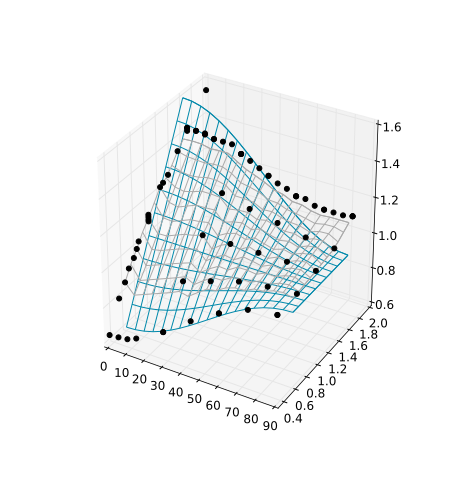
\includegraphics[width=\textwidth]{fig/numvanal.png}
\caption{A comparison of the numerical results and the analytical theory shows
general agreement. Grey dots represent numerical simulation results, the grey surface represents an interpolating surface of the dots, and the blue surface represents the analytical model. Disagreement between the two may be due to edge effects and/or numerical
model convergence issues.}
\label{fig:numvanal}
\end{figure}

Many details may be seen more readily in two-dimensional plots. In particular,
Figure \ref{fig:by_angle} shows theoretical predictions from both the analytical
and numerical model as a function of anisotropic conductivity ratios, sliced by
angle, while Figure \ref{fig:by_kratio} shows theoretical predictions from both
methods as a function of angle, sliced by anisotropic conductivity ratios.
Figure \ref{fig:by_angle} readily shows that an increase in conductivity ratio
above \(1\) has a weaker effect on effective conductivity for the numerical
model than in the analytical model. This may be due to edge effects decreasing
the effective thermal conductivity in the numerical model by conducting heat
axially from the needle. The analytical model, in contrast, does not model edge
effects, as it models an infinitely long needle like the
original needle probe method. For the isotropic case, these edge effects have
been studied and quantified analytically by other researchers. \cite{axialerror}

\begin{figure}[h]
\centering
\includegraphics[width=0.8\textwidth]{fig/byAngle.png}
\caption{Slices of theoretical predictions by angle. Black points connected by dashed lines represent numerical results, while solid blue lines represent analytical theory. It can be seen that the analytical theory predicts measured conductivity to be a stronger function of angle than the numerical data at
higher conductivity ratios.}
\label{fig:by_angle}
\end{figure}

Figure \ref{fig:by_kratio} also shows the smoothing seen in Figure 
\ref{fig:by_angle}, but also readily shows the predictions of both models for
the isotropic case (\(\flatfrac{k_{\textrm{eff}}}{k_{xy}} = 1\)). Both models
correctly predict that effective thermal conductivity is not a function of angle
for the isotropic case. However, it is also clear that the numerical model
over-predicts \(k_{\textrm{eff}}\) by at least \(10\%\). 

The dominant cause for this discrepancy is believed to be due to using a model with too
coarse of a mesh. The convergence study results show that, while the time/temperature curves look
largely the same (Figure \ref{fig:conv_curves}), that the minor differences are magnified when taking the
derivative with respect to \(\ln(t)\) such that the coarse grid reports a
thermal conductivity of about \(110\%\) of the finer grid (Table \ref{tab:conv_kvals}).
This difference is of the same order of magnitude as the difference seen between
the numerical predictions and the analytical predictions, and it is believed that
running the same simulations at a finer grid would resolve most of the difference
seen, particularly in the isotropic case.

However, some of this may also be due to edge effects, as evidenced by the cluster
of points at the zero angle
(More readily seen in Figure \ref{fig:angle0}), where it can be seen that, in fact,
the predictions for the numerical method are a very weak function of \(k_{xy}\)
and not just the ratio of the anisotropic conductivities. Simply repeating the
experiments at higher resolutions of mesh should be able to resolve this problem.

\begin{figure}[h]
\centering
\includegraphics[width=0.8\textwidth]{fig/byKratio.png}
\caption{Slices of theoretical predictions by \(\flatfrac{k_z}{k_{xy}}\). Black points connected by dashed lines represent numerical results, while solid blue lines represent analytical theory. It can be seen that the analytical theory
is perfect for the isotropic case (\(\flatfrac{k_z}{k_{xy}} = 1\)), while the numerical experiments report larger-than-expected values.}
\label{fig:by_kratio}
\end{figure}

\begin{figure}[h]
\centering
\includegraphics[width=0.6\textwidth]{fig/conv_curves.png}
\caption{A comparison of two \(T(t)\) curves from equivalent simulations with 
different fineness of mesh. These two curves appear quite similar, but their long-
time slopes are measurably different}
\label{fig:conv_curves}
\end{figure}


\begin{table}[h]
\centering
\caption{A comparison of \(k_{\textrm{eff}}\) from two equivalent simulations 
with different fineness of mesh. Despite the similarities in time/temperature
curves, the resulting  conductivity calculations differ by nearly 10 \%. Units are in W\(/\)m\(\cdot\)K.}
\begin{tabular}{r | l}
 & Slope\\
\(35892\) elements & 0.215\\
\(159641\) elements & 0.198\\
\% Error & 8.64 \%
\end{tabular}

\label{tab:conv_kvals}
\end{table}

Figure \ref{fig:angle0} shows predictions for the special case of
\(\theta = 0 \), where the needle is oriented parallel to the planes of isotropy.
This special case is of interest because previous needle probe measurements have
determined effective conductivities at this angle, which may or may not be
accurate representations of \(k_z\), the vertical thermal conductivity, which is
what is measured by a guarded hot plate apparatus and is the conductivity
of interest to climatologists modeling heat transfer between the atmosphere and
soil. If predictions for \(k_{\textrm{eff}}\) are \emph{equal} to \(k_z\), then
the measured \(k_{\textrm{eff}}\) accurately reflects \(k_z\). This agreement
between measurements seems unlikely for anisotropic measurements, and in fact 
the numerical model shows the expected trend of \(k_{\textrm{eff}} > k_z\) for
low conductivity ratios, and \(k_{\textrm{eff}} < k_z\) for higher conductivity
ratios. However, the analytical model predicts that \(k_{\textrm{eff}} = k_z\)
for all anisotropy ratios. While the analytical model shows expected behavior
for the isotropic case and shows the general trends one would expect, this
surprising result casts doubt onto the validity of the analytical model.

\begin{figure}[h]
\centering
\includegraphics[width=0.8\textwidth]{fig/angle_0.png}
\caption{Theoretical predictions for the special case of \(\theta = 0 \),
when the needle is oriented horizontally. Blue points represent numerical solution, while green shows the line where \(k_{\textrm{eff}} = k_z\), where measured conductivity and vertical conductivity are the same. The analytical predictions are indistinguishable from this line, and are therefore not plotted.}
\label{fig:angle0}
\end{figure}


\section{Benchtop Measurements}

\begin{figure}[h]
\centering
\includegraphics[width=0.9\textwidth]{fig/test_results.png}
\caption{A comparison of the benchtop measurements with the numerical and
analytical predictions for alternating layers of salt and sugar, given the
calculated anisotropic thermal conductivity.}
\label{fig:test_results}
\end{figure}

\begin{table}[h]
\centering
\caption{Raw data from the benchtop measurements. Note that one of the cooling curve measurements is striked out. This is because, when examined, it is clearly an outlier. Units are in W\(/\)m\(\cdot\)K.}
\begin{tabular}{l l | l l}
Angle (degrees) & \# & Heating & Cooling\\
90 & 1 & 0.223284242942 & 0.243481576262\\
& 2 & 0.246684312618 & 0.24641641198\\
& 3 & 0.255505537961 & \sout{0.318256880271}\\
75 & 1 & 0.212791418373 & 0.223684883264\\
& 2 & 0.2325853424 & 0.232407779425\\
& 3 & 0.207604305022 & 0.225508200642\\
& 4 & 0.22608462065 & 0.237662896347\\
60 & 2 & 0.238543591267 & 0.244064408529\\
& 3 & 0.225850168518 & 0.22374914604\\
& 4 & 0.217518339596 & 0.216990054548\\
30 & 1 & 0.226573190917 & 0.238313150421\\
& 2 & 0.226429675463 & 0.247135960358\\
& 3 & 0.220619372302 & 0.241951060919\\
& 4 & 0.223387867071 & 0.221486604074\\
\end{tabular}

\label{tab:powders}
\end{table}


\begin{figure}[h]
\centering
\includegraphics[width=0.9\textwidth]{fig/test_results_confidence.png}
\caption{Upper and lower bounds of 95 \% confidence in thermal conductivity measurements of the salt and sugar layered samples. This analysis 
indicates that the measurements can not statistically exclude a null hypothesis.}
\label{fig:test_confidence}
\end{figure}

\begin{table}[h]
\centering
\caption{Basic statistics on normalized benchtop measurements.  Units are in W\(/\)m\(\cdot\)K.}
\begin{tabular}{r | l l l}
 & \multicolumn{3}{c}{ \(k_{\textrm{meas}} / \bar{k_{xy}}\) }\\
Angle & Mean & Standard Deviation & 95\% Confidence\\
90 & 1.000 & 0.0491 & 0.0431\\
75 & 0.923 & 0.0419 & 0.0291\\
60 & 0.937 & 0.0459 & 0.0367\\
30 & 0.949 & 0.0420 & 0.0291\\
\end{tabular}

\label{tab:pow_stats}
\end{table}


It may be seen that there is a significant amount of variation between
benchtop measurements using the needle probe method in Figure \ref{fig:test_results} and Table \ref{tab:pow_stats}, even accounting for obviously failed measurements such as the removed outlier in Table \ref{tab:powders}.
This is likely due in part to the nature of numerical derivatives as well as the relatively
unpredictable behavior of porous materials. Given
this variation, it is difficult to see which of the two models (analytical or numerical) is more appropriate.

Based on a general curve fit, the benchtop results show a slight upward slope (Figure \ref{fig:test_results}) as
expected. However, given the variation in the benchtop results, it is statistically
possible that angle has absolutely no effect on the reading. This could be fixed
with more careful, exacting standards in the construction of the anisotropic
materials, more measurements at each angle, and measurements at more angles.
In other words, given the variance of the measurements, many more measurements
would have to be made in order to reach any statistically significant
conclusions, at least given the relatively low amount of anisotropy of the sample.

Also given this variation and the relatively weak levels of anisotropy in the
sample, even with more measurements it could still prove difficult to deduce
the degree of anisotropy of the sample with this data and a curve fit to either
the numerical or analytical predictions alone.

\section{In-Situ Snow Measurements}

% This would be a good thing for an appendix.
\begin{comment}
\begin{table}[h]
\centering
\begin{tabular}{l | l l}
\# & h (inches) & Angle (degrees)
5 & 10.5 & 85\\
6 & 10.5 & 85\\
7 & 13 & 38\\
8 & 12.5 & 45\\
9 & 10.5 & 92
\end{tabular}

\label{tab:metadata}
\caption{Height and angle measurements from snow measurements. The height data was unused in this analysis.}
\end{table}
\end{comment}

\begin{table}[h]
\centering
\caption{Conductivity results from the snow measurements. Units are in W\(/\)m\(\cdot\)K.}
\begin{tabular}{r | l l}
Angle & Heating & Cooling\\
0 & 0.0289001039328 & 0.0320660927581\\
5 & 0.0268615378785 & 0.0244255288984\\
45 & 0.0289529144315 & 0.0326746396833\\
52 & 0.0287736535682 & 0.0326165606258\\
\end{tabular}

\label{tab:snow}
\end{table}

\begin{table}[h]
\centering
\caption{Measured and derived measurements for snow density. Units are in W\(/\)m\(\cdot\)K.}
\begin{tabular}{r | l}
Control Volume & \(736.76\) mL\\
Mass & \(161.14\) g\\
Density & \(0.219\) g/mL\\
& 219 kg/\(\textrm{m}^3\)\\
\end{tabular}

\label{tab:density}
\end{table}

\begin{figure}[h]
\centering
\includegraphics[width=0.9\textwidth]{fig/snow_meas.png}
\caption{Conductivity measurements in roughly the same layer of snow at various 
angles. Even a limited amount of in-situ snow measurements suggest a degree of
anisotropy.}
\label{fig:snow_results}
\end{figure}

\begin{figure}[h]
\centering
\includegraphics[width=0.9\textwidth]{fig/snow_meas_boxplot.png}
\caption{These boxplots give a general idea of the differences in measurements
between the near-horizontal angle and the more oblique ones in snow.}
\label{fig:test_boxplot}
\end{figure}


Due to the difficulty in taking snow measurements, very few snow measurements were
successfully completed (Table \ref{tab:snow}). This, on top of the inherent variation between measurements seen in the method, snow measurements are also inconclusive. However, the
measurements taken \emph{do} indicate anisotropy to a greater degree of confidence
than the benchtop measurements, as may be seen in Figures \ref{fig:snow_results}
 and \ref{fig:test_boxplot}. Like the case of the benchtop measurements, with so few
measurements a curve fit against either method of prediction is unlikely to
yield useful results.

While the degree of anisotropy of the snow sample is unknown, it is known that
the measurements indicate a \(\flatfrac{k_z}{k_xy}\) of less than one, which is
indicative of the aggregate anisotropy seen from a geometry of alternating
layers, and not of the particular structural anisotropy that is seen in some
types of snow such as depth hoar \emph{or} or the sort of anisotropy that could
explain the discrepancies between needle probe and guarded hot plate measurements.
This is not surprising, as the measurements were taken in a layered region in
order to increase the chances of detecting anisotropy.

To put the snow measurements in context for comparison in future studies, Table
\ref{tab:density} shows the snow density in the region of snow
that these measurements were taken.

\section{Ramifications}

These results indicate that anisotropy is possible to measure in snow. However,
due to variance between measurements, this may be more difficult than hoped for.
While only two perfect measurements would likely be required to ascertain the
anisotropic thermal conductivity of snow given a proven model, the variance seen
in these measurements suggests that many more measurements would be
required---somewhere on the order of five to ten measurements per angle would
likely be required for statistically significant results.

However, horizontal measurements do reflect vertical conductivity to a degree,
and for small levels of anisotropy (likely if the anisotropy is on the aggregate
level only) horizontal measurements may be sufficient for ascertaining vertical
conductivity.

Given that anisotropy was detected in the snowpack, it is possible that snow
anisotropy is responsible for the discrepancies between guarded hot plate
measurements and needle probe measurements. However, because aggregate anisotropy
would lead us to predict higher in-plane conductivity than out-of-plane conductivity,
only structural anisotropy can explain this discrepancy.

\chapter{Future Work}

\section{Introduction}

This is clearly not the end of research on this method. While the groundwork has
been laid, there are plenty of avenues which need more study.

\section{Assumptions in the Analytical Approach}

In the analytical model presented here, the needle is assumed to be of zero
thickness, and yet an average temperature over an ellipse is taken which
represents the needle surface.  The model seems to work; however, there are
other way to represent such a problem that may yield more accurate results. For
example, one may be able to approach the problem in terms of a needle with a
finite thickness, in which case the solution to the problem should be an
infinite series of Bessel functions in the isotropic case. One may be able to
tackle the problem from a finite-thickness needle approach for better results. In addition, a refined model could account for edge effects. \cite{axialerror}

\section{Extended Convergence Study}

While a convergence study for the numerical model was undertaken, it was relatively
informal, and executed for only one particular configuration of parameters. A
more thorough investigation of the convergence properties of the numerical model
should likely be undertaken.

\section{Improved Benchtop Method}

The benchtop apparatus was based on the use of glycerine and agar gels for
calibration. However, the current anisotropic benchtop method uses sugar and
salt. This makes the proper layering of the materials difficult. Moreover, the
device is limited to a tilt factor of \(30\) degrees from horizontal due to the
location of the bottle's opening. Presumably, this method could be improved upon
to allow for more accurate material layering and for an increased range of
needle angles.

In addition, the materials used only lend themselves to an anisotropy ratio of
87\%. There is plenty of room for improvement, in terms of suitable materials.
Figure \ref{fig:anisovmatl_rats} shows what material conductivity ratios are
required to achieve a given anisotropic conductivity ratio, assuming
equal-thickness layers, which achieves the most extreme anisotropy ratio for
two given materials and an alternating-layers configuration. While salt and
sugar fare poorly, real-world materials have a wide range of conductivities
such that two materials with sufficiently different conductivities should be
possible to find.

\begin{figure}[h]
\centering
\includegraphics[width=0.7\textwidth]{fig/anisovmaterial_ratios.png}
\caption{Anisotropic Conductivity Ratio vs. Material Conductivity Ratio for the
layered geometry used in the benchtop experiments. It may take a very large
material conductivity ratio in order to achieve a relatively minor anisotropic
conductivity ratio.}
\label{fig:anisovmatl_rats}
\end{figure}

\section{Comprehensive Benchtop Measurements}

While enough benchtop measurements were taken to give a vague idea as to the
effectiveness of this measurement technique, there were not nearly enough
measurements to give a statistically valid conclusion regarding the slight
trend we were looking for. In addition to improving the benchtop method, there
need to be many more measurements taken, in order to draw statistically valid
conclusions.

\section{Comprehensive In-Situ Measurements}

The in-situ measurements presented in this document are very limited in scope.
One could easily spend much more time taking more measurements on more snow at
more angles, in order to better quantify the degrees of anisotropy in natural
snowpacks. More measurements would allow for a rigorous statistical analysis that
can show a trend with high confidence.


\section{Exploration of the Cooling Curve}

In the numerical and analytical models, the cooling curve is all but ignored. It
is believed that cooling curve models will yield analogous results, but this has
not been tested. Because of the importance of cooling curve measurements in the
real world (as they effectively double the number of measurements in a sample),
verification of these expectations of analogous behavior should occur.

\section{A Method for Determining Anisotropic Thermal Conductivity From Measurements}

While this document lays the groundwork for determining anisotropic thermal
conductivity from measurements, a reliable method for converting measurements
into anisotropic thermal conductivities has not been found. Were the data
more reliable and less variable, one may be able to find the portion of the
prediction curve(s) that best fit the data, but based on current measurements,
this doesn't seem likely.

One possibility is that, instead of focusing on the measured conductivities as a
function of angle, that one should focus on the \emph{change} in measured
conductivities with respect to angle. In fact, given low enough degrees of
anisotropy, it may be sufficient to compare linearizations of these curves. Only
with more research can this conjecture be shown to be valid.

\chapter{Conclusions}

An analytical model based on the isotropic solution outlined by
Carslaw and Yeager has been modified in order to predict thermal conductivity
measurements of anisotropic materials as a function of insertion angle.  This
model uses a linear transformation to pose the problem in a form equivalent to
the isotropic problem. However, in order to get meaningful results, the model
requires calculating the average temperature along an ellipse.

A 3-D finite element numerical model has also been built in order to predict
thermal conductivity measurements  of anisotropic materials as a function of
insertion angle. While the base model is simple by finite element model
standards, the number of parameters iterated through is somewhat unusual for
finite element modeling, and taxes the abilities of the software used.

According to both numerical and analytical theories, anisotropic thermal
conductivity should cause predictable changes in needle probe heating curve
measurements as a function of angle. While the two models show general
agreement, there are significant differences between the two predictions. These
may be explained by the 3D model's handling of edge effects, as well as possible
issues with the numerical model's convergence properties.

Measurements of engineered anisotropic materials are promising, but far from
complete. A basic, repeatable method has been designed and tested. The initial
results indicate the expected trend; however, due to the relatively low
amount of anisotropy in the material, the inherent noise in the thermal
conductivity measurement method and a disappointingly low amount of
measurements, a null hypothesis is impossible to rule out.

Similarly, in-situ measurements of snow have been made, but due to difficulties
in snow measurement very few useful data points were collected. However, the
results do suggest anisotropy in the snow.

Unfortunately, inquiry on this method is far from complete. Aside from the need
for more measurements, there are plenty of avenues for future researchers to
study. These include updating and refining the methods, studying cooling curves,
and analyzing the current models with increased scrutiny.


\bibliographystyle{agufull08}
\bibliography{thesis}

\appendix
\chapter{Code Used in Chapter \ref{sec:analytical-np}}
\label{apx:analytical-np}

\section{model.py}

\small
\begin{minted}{python}
import json
from math import pi
from numpy import log, sin, cos, sqrt, array, \
                  arange, hstack, linspace, dot
from functools import reduce

def elliptical(fxn, ecc):
    from scipy.integrate import quad
    from math import pi
    from numpy import sin, cos, sqrt
    from types import FunctionType, BuiltinFunctionType

    #API trickery.
    if type(fxn) != FunctionType and type(fxn) != BuiltinFunctionType:
        fxn2 = lambda ecc, th: fxn
    else:
        fxn2 = fxn

    #The heavy lifting.
    return quad(lambda th: fxn2(ecc,th) *
                               sqrt( cos(th)**2.0 + (ecc*sin(th))**2.0 ),
                0, 2*pi)[0]

def Tavg(k_x, k_y, q, t):
    """
    given scalar r0, k_x, k_y and 1-d time, this returns a curve with
    the same slope at Tavg(t) for long T. May refactor.
    """
    return (4*pi*k_x/q)*array([elliptical(log(time) , k_x/k_y)/
                               elliptical(1, k_x/k_y) for time in t])

def kmeas(k_x, k_y, q, t):
    from numpy import polyfit
    """
    Does a quick linear curve fit 
    """
    return (q/4/pi)*polyfit(log(t), Tavg(k_x, k_y, q, t), 1)[0]


def rot(th, axis):
    from numpy.linalg import norm
    from numpy import sin, cos, eye, outer, cross
    if axis == "x":
        axis = array([1,0,0])
    elif axis == "y":
        axis = array([0,1,0])
    elif axis == "z":
        axis = array([0,0,1])
    else:
        axis = axis/norm(axis)
    oh = outer(axis, axis)
    return oh + cos(th)*(eye(3) - oh) + sin(th)*cross(axis, eye(3))
    

def proj(matrix, rot):
    from numpy import eye, hstack, vstack, newaxis
    from numpy.linalg import eig
    return tuple(
               eig(
                   reduce( dot, [ vstack((
                                    hstack((
                                        eye(2),
                                        array([0, 0])[:, newaxis] )),
                                    array([0, 0, 0]))),
                                    rot,
                                    matrix,
                                    rot.T ]))[0])[0:2]


if __name__=="__main__":
    from numpy import diag, logspace, meshgrid
    from math import pi
    from progressbar import ProgressBar

    angles = range(0, 91) # Lots angles :D

    ks = arange(0.2, 0.4, 0.05) # Some ks
    (k_xy, k_z) = meshgrid(ks, ks)
    k_xy = k_xy.flatten()
    k_z = k_z.flatten()

    q = 0.5 #Like in sims
    t = hstack(( logspace(0.1,1.0,15),
                 logspace(1.0,3.0,15) ))

    results = []
    progress = ProgressBar()
    for th in progress(angles):
        for i in xrange(k_xy.shape[0]):
            (k_xp, k_yp) = proj( diag([k_xy[i], k_xy[i], k_z[i]]),
                                 rot(pi/180*(90-th), 'y'))
            results.append([ th,
                             k_z[i]/k_xy[i],
                             kmeas(k_xp, k_yp, q, t)/k_xy[i]])
    for row in results:
        print(', '.join(map(str, row)))
\end{minted}
\normalsize

\chapter{Code Used for Chapter \ref{ch:numerical-np}}
\label{apx:numerical-np}

\section{worker.m}
\small
\begin{minted}{matlab}
%worker.m
%does the working

function worker(kxy,kz)
    load('angles.mat', 'angles');
    angles
    [kxy,kz] = meshgrid(kxy,kz);

    % The commented-out ``flreport'' gives one the option of suppressing
    % graphical output from COMSOL. This is useful if one wants to run COMSOL in
    % a headless manner. Unfortunately, COMSOL 3.5a on the ARSC systems has
    % extreme difficulties running in headless batch mode.
    %flreport('off');

    params=struct('rsnow', 0.4, ...
                  'rneedle', 0.00025, ...
                  'lneedle', 0.1, ...
                  'density_snow', 200, ...
                  'density_needle', 8000, ...
                  'cp_snow', 2050, ...
                  'cp_needle', 460, ...
                  'q_needle', 0.5, ...
                  'k_needle', 160, ...
                  'time', [logspace(0.1,1,15) logspace(1,3,15)], ...
                  'angles', angles );

    saveroot=['./solutions-' date '/'];

    mesh = mesher(0,params);
    for angle=angles,
        try
            solutions = arrayfun(@(x,y) solver(x,y,mesh,angle,params), ...
                            kxy,kz, 'UniformOutput', false);
            save solutions
            fprintf('Fitting solutions...\n');
            solutions = {cellfun(@(tsd) {fitter(tsd{1}(1,:),tsd{1}(2,:), ...
                                             0.999,params), ...
                             tsd{1}, tsd{2}}, ...
                         solutions, 'UniformOutput', false)};
            fprintf('A solution set just completed.');
            system([ 'echo "A solution set finished on" `hostname` ' ...
                     '| mutt -s "A solution set completed." ' ...
                     'josh.holbrook@gmail.com' ]);
        catch exception
            system([ 'echo "Exception occurred on" `hostname` ' ...
                     '| mutt -s "Exception occurred--' exception.message ...
                     '" josh.holbrook@gmail.com' ]);
        end
        angles = angles(2:length(angles));
        save('angles.mat', 'angles');
        %solutions
        mkdir(saveroot);
        save([ saveroot 'solution-' num2str(angle) ], ...
             'solutions','angle','kxy','kz','params');
    end

    % Emails me when everything's done
    system([ 'echo "Results completed on " `hostname` ' ...
             '| mutt -s "Results Completed" ' ...
             'josh.holbrook@gmail.com' ]);
    system('touch down');
end
\end{minted}
\normalsize


\section{mesher.m}
\small
\begin{minted}{matlab}
% COMSOL Multiphysics Model M-file
% Generated in part by COMSOL 3.5a (COMSOL 3.5.0.608, $Date: 2009/05/11 07:38:49 $)
% the rest of it modified by Joshua Holbrook

function fem=mesher(angle,params)
    % mesh_generate(angle)
    % generates a mesh for the given angle. 

    fprintf(['meshing for angle=' num2str(angle) '...\n']);
    flclear fem

    % COMSOL version
    clear vrsn
    vrsn.name = 'COMSOL 3.5';
    vrsn.ext = 'a';
    vrsn.major = 0;
    vrsn.build = 608;
    vrsn.rcs = '$Name: v35ap $';
    vrsn.date = '$Date: 2009/05/11 07:38:49 $';
    fem.version = vrsn;

    % Geometry
    g1=sphere3(num2str(params.rsnow),'pos',{'0','0','0'},'axis',{'0','0','1'},'rot','0');
    g2=cylinder3(num2str(params.rneedle),num2str(params.lneedle),'pos',{num2str(-params.lneedle/2),'0','0'},'axis',{'1','0','0'},'rot','0');
    parr={point3(0,0,0)};
    g3=geomcoerce('point',parr);
    parr={point3(params.rsnow,0,0)};
    g4=geomcoerce('point',parr);
    parr={point3(0,params.rsnow,0)};
    g5=geomcoerce('point',parr);
    parr={point3(0,0,params.rsnow)};
    g6=geomcoerce('point',parr);
    parr={point3(-params.rsnow,0,0)};
    g7=geomcoerce('point',parr);
    parr={point3(0,-params.rsnow,0)};
    g8=geomcoerce('point',parr);
    parr={point3(0,0,-params.rsnow)};
    g9=geomcoerce('point',parr);

    % Analyzed Geometry (?)
    clear p s
    p.objs={g3,g4,g5,g6,g7,g8,g9};
    p.name={'ORIGIN','PT1','PT2','PT3','PT4','PT5','PT6'};
    p.tags={'g3','g4','g5','g6','g7','g8','g9'};

    s.objs={g1,g2};
    s.name={'SNOW','NEEDLE'};
    s.tags={'g1','g2'};

    fem.draw=struct('p',p,'s',s);
    fem.geom=geomcsg(fem);


    % ODE Settings
    clear ode
    clear units;
    units.basesystem = 'SI';
    ode.units = units;
    fem.ode=ode;


    % Initialize mesh
    fem.mesh=meshinit(fem, ...
                      'hauto',5, ...
                      'hgradsub',[2,1.1], ...
                      'hmaxsub',[2,0.0005]);

    % Refine mesh
    fem.mesh=meshrefine(fem, ...
                        'mcase',0, ...
                        'rmethod','longest');

    fem=multiphysics(fem);
end
\end{minted}
\normalsize

\section{solver.m}
\small
\begin{minted}{matlab}
% COMSOL Multiphysics Model M-file
% Generated by COMSOL 3.5a (COMSOL 3.5.0.608, $Date: 2009/05/11 07:38:49 $)

function answer=solver(kxy,kz,fem,theta,params)
    %solver(kxy,kz,mesh,params)
    %uses comsol to pump out a solution using a given mesh-mat and a k-matrix in comsol format.

    fprintf(['solving for kxy=' num2str(kxy) ' and kz=' num2str(kz) '...\n']);
    % Application mode 1
    clear appl
    appl.mode.class = 'GeneralHeat';
    appl.module = 'HT';
    appl.shape = {'shlag(1,''J'')','shlag(2,''T'')'};
    appl.sshape = 2;
    appl.assignsuffix = '_htgh';
    clear bnd
    bnd.type = {'q0','cont'};
    bnd.shape = 1;
    bnd.ind = [1,1,1,1,2,2,2,2,2,1,1,1,1,2];
    appl.bnd = bnd;
    clear equ
    equ.sdtype = 'gls';
    % densities
    equ.rho = {params.density_snow,params.density_needle};
    equ.init = 0;
    equ.shape = 2;
    % Heat capacities
    equ.C = {params.cp_snow,params.cp_needle};
    % Wattage
    equ.Q = {0,params.q_needle/pi/(params.rneedle)^2};
    % Heat conductivities
    arr = [cos(theta*pi/180), 0, sin(theta*pi/180); 0, 1, 0; -sin(theta*pi/180), 0, cos(theta*pi/180)]; %rotation matrix
    equ.k = {symmetric_tocell(arr*diag([kxy,kxy,kz])*(arr')),params.k_needle};
    equ.ind = [1,2];
    appl.equ = equ;
    fem.appl{1} = appl;
    fem.frame = {'ref'};
    fem.border = 1;
    fem.outform = 'general';
    clear units;
    units.basesystem = 'SI';
    fem.units = units;

    % Coupling variable elements
    clear elemcpl
    % Integration coupling variables
    clear elem
    elem.elem = 'elcplscalar';
    elem.g = {'1'};
    src = cell(1,1);
    clear bnd
    bnd.expr = {{'T',{}},{'1',{}}};
    bnd.ipoints = {{'4',{}},{'4',{}}};
    bnd.frame = {{'ref',{}},{'ref',{}}};
    bnd.ind = {{'1','2','3','4','10','11','12','13'},{'5','6','7','8','9', ...
      '14'}};
    src{1} = {{},{},bnd,{}};
    elem.src = src;
    geomdim = cell(1,1);
    geomdim{1} = {};
    elem.geomdim = geomdim;
    elem.var = {'int_T','area'};
    elem.global = {'1','2'};
    elemcpl{1} = elem;
    fem.elemcpl = elemcpl;

    % ODE Settings
    clear ode
    clear units;
    units.basesystem = 'SI';
    ode.units = units;
    fem.ode=ode;

    % Multiphysics
    fem=multiphysics(fem);

    % Generate GMG mesh cases
    fem=meshcaseadd(fem,'mgauto','anyshape');

    % Extend mesh
    fem.xmesh=meshextend(fem);

    % Solve problem
    fem.sol=femtime(fem, ...
                    'solcomp',{'T'}, ...
                    'outcomp',{'T'}, ...
                    'blocksize','auto', ...
                    'tlist', params.time, ...
                    'estrat',1, ...
                    'tout','tlist', ...
                    'linsolver','gmres', ...
                    'itrestart',100, ...
                    'prefuntype','right', ...
                    'prefun','gmg', ...
                    'prepar',{'presmooth','ssor','presmoothpar',{'iter',3,'relax',0.8},'postsmooth','ssor','postsmoothpar',{'iter',3,'relax',0.8},'csolver','pardiso'}, ...
                    'stopcond','0.06-int_T/area', ...
                    'mcase',[0 1]);

    % Save current fem structure for restart purposes
    fem0=fem;

    % Plot solution
    %{
    postplot(fem, ...
             'slicedata',{'T','cont','internal','unit','K'}, ...
             'slicexspacing',5, ...
             'sliceyspacing',0, ...
             'slicezspacing',0, ...
             'slicemap','Rainbow', ...
             'solnum','end', ...
             'title','Time=100    Slice: Temperature [K]', ...
             'grid','on', ...
             'campos',[-2.636014311828346,-3.4353207343472505,2.4999999999999996], ...
             'camtarget',[0,0,0], ...
             'camup',[0,0,1], ...
             'camva',41.213465344831754);
    %}

    % Integrate
    T_thermistor=postint(fem,'T', ...
               'unit','K', ...
               'recover','off', ...
               'dl',8, ...
               'edim',0, ...
               'solnum','all');

    % Integrate
    T_surf_avg=postint(fem,'T', ...
               'unit','', ...
               'recover','off', ...
               'dl',[1,2,3,4,10,11,12,13], ...
               'edim',2, ...
               'solnum','end');

    answer={[fem.sol.tlist; T_thermistor],T_surf_avg};
    angles = params.angles(2:length(params.angles));
    %fprintf([ '''' kxy '; ' kz '; ' theta '; ' fem.sol.tlist '; ' T_thermistor '; ' T_surf_avg ''' >> results.txt' ]);
    %system([ '''' kxy '; ' kz '; ' theta '; ' fem.sol.tlist '; ' T_thermistor '; ' T_surf_avg ''' >> results.txt' ]);

    %flsave(['fem-' num2str(theta) '-' num2str(kxy) '-' num2str(kz) '.mph']);

    save('angles.m', 'angles');
end
\end{minted}
\normalsize

\section{fitter.m}
\small
\begin{minted}{matlab}
function k = fitter(t,T,rset,params)
    logt = log(t(t>1));
    T = T(t>1);

    disp('Finding linear portion...');    
    for i=1:length(logt)-1
        C = corrcoef(logt(i:length(logt)), T(i:length(T)));
        r = sqrt(C(2,1));
        if r > rset %adjust this to get 'good' values
            disp(['linear fitting to ' num2str((length(logt)-i)) ' points from t=' num2str(exp(logt(i))) ' to t=' num2str(exp(logt(length(logt)))) '...']);
            x = polyfit(logt(i:length(logt)),T(i:length(T)), 1);
            break
        end
    end

    %plot(logt,T,'*');
    %hold on;
    %plot(logt, x(1)*logt + x(2));
    k = (params.q_needle)/(4*pi*x(1));

end
\end{minted}
\normalsize

\section{assembler.m}
\small
\begin{minted}{matlab}
function answers=assembler(directory)
    cd(directory);
    d = dir();
    answers = [];
    for i=3:length(d),
        disp(['Opening ' d(i).name '...']);
        load(d(i).name);
        answers = [answers, solutions];
    end
    cd('..');
end
\end{minted}
\normalsize

\section{reFitter.m}
\small
\begin{minted}{matlab}
function fixed=reFitter(broked, r, params)
    fixed = broked;
    for i=1:length(fixed),
        fixed{i} = cellfun(@(kset) {fitHelper(kset{2}, r, params), kset{2}, kset{3}}, fixed{i}, 'UniformOutput', false);
    end
end

function fitted=fitHelper(tT, r, params)
    fitted = fitter(tT(1,:),tT(2,:),r, params);
end
\end{minted}
\normalsize

\section{analyzer.m}
\small
\begin{minted}{matlab}
%analyzer
%Does some analyzing of the simulation results
%breaks for [kxy,kz] != meshgrid(ks,ks)

%Solutions location
%load solutions-19-Sep-2010/solutions-all.mat;

%Things I already know :)
%ks = linspace(0.2, 0.4, 6);
%ks = [0.2,0.4];
%[kxy, kz] = meshgrid(ks, ks);
%[kzy, kz] = meshgrid(0.3, 0.5);
%ks = 1;
%angles = 0:15:90;
%angles = 0:5:90;
%angles = [0 90];

%For an obvious color gradient, from red to blue right now.
colores = @(i,n) [sin((i/n)*pi/2), 0, cos((i/n)*pi/2)];

disp('Showing overlaid plots (YES ALL OF THEM) to make sure they "look" right:');
figure;
hold on;
for theta = 1:length(angles)
    for i=1:length(ks)^2
        tT = answers{theta}{i}{2};
        plot(log(tT(1,tT(1,:) > 1 )),tT(2,tT(1,:) > 1), 'color', colores(i,length(ks)^2));
    end
end

disp('Sanity checking results for isotropic cases');
figure;
hold on;
kmsold = 0 * cellfun(@(prison) prison{1}, answers{1});
for i=1:length(angles)
    %Extracts all the measured k's from the data
    % "prison" refers to cell representing particular k combination in answers{theta}
    kms = cellfun(@(prison) prison{1}, answers{i});
    if kms == kmsold,
        disp('wtf exactly equivalent kms''s');
    end
    %diag(kms)
    %diag(kxy)
    errs = 100*(diag(kms) - diag(kxy))./diag(kxy);
    %Not necessary to be 3d anymore :)
    plot3(diag(kxy), errs, angles(i)*ones(size(diag(kxy))), '*-', 'color', colores(i,length(angles)) );
    xlabel('k_{actual}');
    ylabel('error (%)');
    zlabel('angle (degrees)');
end

disp('Figuring out T_surf_avg at time T:');
%figure;
%hold on;
for theta=1:length(angles)
    tavgs = cellfun(@(prison) prison{3}, answers{theta});
    try
        assert(all(all(tavgs< 0.001)));
    catch
        disp(['Warning: average surface temps are a bit high at theta=' num2str(angles(theta))] );
        disp(tavgs);
    end
    if theta == length(angles)
        figure;
        hold on;
        contourf(kxy,kz,tavgs);
        colorbar;
        colormap('pink');
        title('Average Surface Temperature at End of Heating Curve Simulation for a representative angle');
        xlabel('K_{xy}');
        ylabel('K_{zz}');
    end
end

%dimensions changed to be in order kxy, then rows are angle and columns are kzz
disp('Plotting k_{meas}/k_{xy} vs. \theta and k_{z}/k_{xy}...');
kms=cell(size(ks));
for i=1:length(angles)
    kmsbyangle = cellfun(@(prison) prison{1}, answers{i});
    for j=1:length(ks)
        kms{j} = [kms{j}; kmsbyangle(:,j)'/ks(j)]; %Normalize by particular kxy
    end
end
figure;
hold on;
[kgrid, anggrid] = meshgrid(ks, angles);
for n=1:length(ks)
    x = reshape(anggrid',[],1), reshape(kgrid'/ks(n),[],1)
    y = reshape(kms{n}',[],1)
    plot3(x, y, '*-', 'color', colores(n, length(ks)));
end
%legend(arrayfun(@(x) num2str(x),ks, 'UniformOutput', false));
xlabel('angle (degrees)');
ylabel('k_{zz}/k_{xy}');
zlabel('k_{meas}/k_{xy}');
\end{minted}
\normalsize

\section{tabulator.m}
\small
\begin{minted}{matlab}
%tabulator
%turns lame structures into some csv action

%given params:
%  answers
%  angles
%  kxy
%  kz

% Bad style, but I'm dealing with a cluttered namespace because I'm not functionalizing these.
% This is because parameter passing is a pita. So, leave me alone.
[Kxy, Kz] = meshgrid(kxy, kz);

fprintf('angle, kxy, kz, kmeas \n');
for t=1:length(angles),
    for pt=1:size(Kxy,1)*size(Kxy,2),
        fprintf([ num2str(angles(t)) ', ' num2str(Kxy(pt)) ', ' num2str(Kz(pt)) ', ' num2str(answers{t}{pt}{1}) '\n']);
    end
end
\end{minted}
\normalsize

\section{symmetric\_tocell.m}
\small
\begin{minted}{matlab}
function a=symmetric_tocell(A)
    % Converts a symmetric matrix A into a cell containing the values, comsol-style.
    %I need to make sure comsol likes them nx1 instead of 1xn.

    %test for squareness
    assert(size(A,1)==size(A,2), 'Dawg that matrix aint square much less symmetric');
    %test for symmetry
    for i=1:size(A,1),
        for j=i:size(A,1),
            if (A(i,j)~=A(j,i)),
                disp(['Warning: Dawg that matrix aint square (A(' int2str(i) int2str(j) ')=' num2str(A(i,j)) ' != A(' int2str(j) int2str(i) ')=' num2str(A(j,i)) ' ! )']);
            end
        end
    end

    %The actual heavy lifting.
    a={};
    for m=1:size(A,1),
        for element=A(1:m,m)' %Takes upper-triangular section of mth column
            a{size(a,1)+1,1}=element;
        end
    end

end

function t=triangle(n)
    t=(n^2+n)/2;
end
\end{minted}
\normalsize


\include{apx3}
\section{Raw Results of Numerical Model}

\begin{table}
\caption{\(\theta = [0:5:90]\), \([k_{xy}, k_z] = [0.3, 0.5]\)}
\begin{tabular}{r l l | l}
Angle (degrees) & \(k_{xy}\) & \(k_z\) & \(k_{\textrm{meas}}\)\\
0 & 0.3 & 0.5 & 0.42503\\
5 & 0.3 & 0.5 & 0.42439\\
10 & 0.3 & 0.5 & 0.42439\\
15 & 0.3 & 0.5 & 0.41927\\
20 & 0.3 & 0.5 & 0.41927\\
25 & 0.3 & 0.5 & 0.41927\\
30 & 0.3 & 0.5 & 0.40758\\
35 & 0.3 & 0.5 & 0.40047\\
40 & 0.3 & 0.5 & 0.39267\\
45 & 0.3 & 0.5 & 0.38462\\
50 & 0.3 & 0.5 & 0.37641\\
55 & 0.3 & 0.5 & 0.37196\\
60 & 0.3 & 0.5 & 0.36418\\
65 & 0.3 & 0.5 & 0.36418\\
70 & 0.3 & 0.5 & 0.35754\\
75 & 0.3 & 0.5 & 0.35574\\
80 & 0.3 & 0.5 & 0.35574\\
85 & 0.3 & 0.5 & 0.35574\\
90 & 0.3 & 0.5 & 0.3589\\
\end{tabular}
\end{table}


\begin{table}
\caption{\(\theta=0\), \([k_{xy}, k_z] = \textrm{meshgrid}(\textrm{linspace}(0.2, 0.4, 4), \textrm{linspace}(0.2, 0.4, 4))\)}
\begin{tabular}{r l l | l}
Angle (degrees) & \(k_{xy}\) & \(k_z\) & \(k_{\textrm{meas}}\)\\
0 & 0.2 & 0.2 & 0.21614\\
0 & 0.2 & 0.26667 & 0.2492\\
0 & 0.2 & 0.33333 & 0.28009\\
0 & 0.2 & 0.4 & 0.30801\\
0 & 0.26667 & 0.2 & 0.25315\\
0 & 0.26667 & 0.26667 & 0.29095\\
0 & 0.26667 & 0.33333 & 0.32668\\
0 & 0.26667 & 0.4 & 0.35519\\
0 & 0.33333 & 0.2 & 0.28594\\
0 & 0.33333 & 0.26667 & 0.32836\\
0 & 0.33333 & 0.33333 & 0.36839\\
0 & 0.33333 & 0.4 & 0.40493\\
0 & 0.4 & 0.2 & 0.31911\\
0 & 0.4 & 0.26667 & 0.36629\\
0 & 0.4 & 0.33333 & 0.40706\\
0 & 0.4 & 0.4 & 0.44717\\
\end{tabular}
\end{table}

\begin{table}
\caption{\(\theta=[30:15:90]\), \(k_{xy} = 0.3\), \(k_z = [0.1:0.1:0.5]\)}
\begin{tabular}{r l l | l}
Angle (degrees) & \(k_{xy}\) & \(k_z\) & \(k_{\textrm{meas}}\)\\
30 & 0.3 & 0.1 & 0.23\\
30 & 0.3 & 0.2 & 0.28322\\
30 & 0.3 & 0.3 & 0.3296\\
30 & 0.3 & 0.4 & 0.3704\\
30 & 0.3 & 0.5 & 0.40758\\
45 & 0.3 & 0.1 & 0.26424\\
45 & 0.3 & 0.2 & 0.29853\\
45 & 0.3 & 0.3 & 0.3296\\
45 & 0.3 & 0.4 & 0.35806\\
45 & 0.3 & 0.5 & 0.38462\\
60 & 0.3 & 0.1 & 0.29307\\
60 & 0.3 & 0.2 & 0.31317\\
60 & 0.3 & 0.3 & 0.3296\\
60 & 0.3 & 0.4 & 0.34888\\
60 & 0.3 & 0.5 & 0.36418\\
75 & 0.3 & 0.1 & 0.31449\\
75 & 0.3 & 0.2 & 0.32006\\
75 & 0.3 & 0.3 & 0.3296\\
75 & 0.3 & 0.4 & 0.33925\\
75 & 0.3 & 0.5 & 0.35574\\
90 & 0.3 & 0.1 & 0.32201\\
90 & 0.3 & 0.2 & 0.32375\\
90 & 0.3 & 0.3 & 0.3296\\
90 & 0.3 & 0.4 & 0.33566\\
90 & 0.3 & 0.5 & 0.3589\\
\end{tabular}
\end{table}

\begin{table}
\caption{\(\theta=[0:30:90]\), \(k_{xy} = 0.3\), \(k_z = [0.1, 0.5]\)}
\begin{tabular}{r l l | l}
Angle (degrees) & \(k_{xy}\) & \(k_z\) & \(k_{\textrm{meas}}\)\\
0 & 0.3 & 0.1 & 0.19287\\
0 & 0.3 & 0.5 & 0.42503\\
30 & 0.3 & 0.1 & 0.23\\
30 & 0.3 & 0.5 & 0.40758\\
60 & 0.3 & 0.1 & 0.29307\\
60 & 0.3 & 0.5 & 0.36418\\
90 & 0.3 & 0.1 & 0.32201\\
90 & 0.3 & 0.5 & 0.3589\\
\end{tabular}
\end{table}

\begin{table}
\caption{\(\theta=[5:5:15]\), \(k_{xy} = 0.3\), \(k_z = [0.1, 0.5]\)}
\begin{tabular}{r l l | l}
Angle (degrees) & \(k_{xy}\) & \(k_z\) & \(k_{\textrm{meas}}\)\\
5 & 0.3 & 0.1 & 0.19429\\
5 & 0.3 & 0.5 & 0.42439\\
10 & 0.3 & 0.1 & 0.19643\\
10 & 0.3 & 0.5 & 0.42247\\
15 & 0.3 & 0.1 & 0.20301\\
15 & 0.3 & 0.5 & 0.41927\\
\end{tabular}
\end{table}


\end{document}
